\documentclass[10pt, a4paper, landscape]{extarticle}

% -----packages-----
\usepackage{multicol} % for multiple columns
\usepackage[landscape]{geometry} % for landscape
\usepackage{parskip} % remove text indentation
\usepackage{graphicx} % for scale tables
\usepackage[compact]{titlesec} % titles spacing
\usepackage{enumitem} % indent of lists
\usepackage{tikz} % for plots
\usepackage{hyperref} % for hyperlinks
\usepackage{amsmath}

% -----page customization-----
\geometry{top=1cm,left=1cm,right=1cm,bottom=1cm} % margins configuration
\pagenumbering{gobble} % remove page numeration
\setlength{\parskip}{0cm} % paragraph skip length
% title spacing:
\titlespacing{\section}{0pt}{2ex}{1ex}
\titlespacing{\subsection}{0pt}{1ex}{0ex}
\titlespacing{\subsubsection}{0pt}{0.5ex}{0ex}

% -----document-----
\begin{document}
\begin{multicols}{3} % set page columns to 3

\begin{center}
\textbf{\LARGE Econometrics Cheat Sheet} \\ {\footnotesize By Marcelo Moreno - King Juan Carlos University} \\ {\footnotesize \href{https://github.com/marcelomijas/econometrics-cheatsheet}{Version 1.2-en}}
\end{center}

\section*{Basic concepts}
\subsection*{Definitions}

\textbf{Econometrics} - is a social science discipline with the objective of quantify the relationships between economic agents, contrast economic theories and evaluate and implement government and business policies.

\textbf{Econometric model} - is a simplified representation of the reality to explain economic phenomena.

\subsection*{Data types}

\textbf{Cross section} - data taken at a given moment in time, an static ``photo". Order does not matter.

\textbf{Temporal series} - observation of one/many variable/s across time. Order does matter.

\textbf{Panel data} - consist of a temporal series for each observation of a cross section.

\textbf{Pooled cross sections} - combines cross sections from different temporal periods.

\subsection*{Phases of an econometric model}

\begin{enumerate}[leftmargin=*]
\setlength{\multicolsep}{0pt}
\begin{multicols}{2}
\item Specification.
\item Estimation.
\columnbreak
\item Validation.
\item Utilization.
\end{multicols}
\end{enumerate}

\subsection*{Regression analysis}
Study and predict the mean value of a variable (dependent variable, $y$) regarding the base of fixed values of other variables (independent variables, $x$'s). In econometrics it is common to use Ordinary Least Squares (OLS) for regression analysis.

\subsection*{Correlation analysis}
The correlation analysis not distinguish between dependent and independent variables.

\begin{itemize}[leftmargin=*]
\item The simple correlation measures the grade of linear association between two variables.
\item The partial correlation measures the grade of linear association between two variables controlling a third variable.
\end{itemize}

\columnbreak

\section*{Assumptions and properties}
\subsection*{Econometric model assumptions}

Under this assumptions, the estimators of the OLS parameters will present good properties. \textbf{Gauss-Markov assumptions extended}:

\begin{enumerate}[leftmargin=*]
\item \textbf{Parameters linearity}. $y$ must be a linear function of the $\beta$'s
\item \textbf{Random sampling}. The sample from the population has been randomly taken. (ONLY makes sense when data is cross section)
\item \textbf{No perfect collinearity}.
\begin{itemize}[leftmargin=*]
\item There are no independent variables that are constant: $Var(X) \neq 0$.
\item There is not an exact linear relation between independent variables.
\end{itemize}
\item \textbf{Conditional mean zero and correlation zero}.
\begin{itemize}[leftmargin=*]
\item There are no systematic errors: $E(u | x_1, ..., x_k) = E(u) = 0$.
\item There are no relevant variables left out the model: $Cov(x_j | u) = 0$ for any $j = 1, ..., k$.
\end{itemize}
\item \textbf{Homoscedasticity}. The variability of the residual is the same for all levels of $x$: $Var(u | x_1, ..., x_k) = \sigma^2$.
\item \textbf{No auto-correlation}. The residuals do not contain information about other residuals: $Corr(u_t, u_s | X) = 0$ for any $t \neq s$. (ONLY makes sense when data is temporal series)
\item \textbf{Normality}. The residuals are independent and identically distributed: $u \sim N(0,\sigma^2)$.
\item \textbf{Data size}. The number of observations available must be greater than $(k + 1)$ parameters to estimate. (Do NOT makes sense under asymptotic situations)
\end{enumerate}

\subsection*{Asymptotic properties of OLS}

Under the econometric model assumptions and the Central Limit Theorem:
\begin{itemize}[leftmargin=*]
\item Hold 1 to 4: OLS is \textbf{unbiased}. $E(\hat{\beta}_j) = \beta_j$
\item Hold 1 to 4: OLS is \textbf{consistent}. $plim(\hat{\beta}_j) = \beta_j$
\item Hold 1 to 5: \textbf{asymptotic normality} of OLS (then, 7 is necessarily satisfied): $u \sim_a N(0,\sigma^2)$.
\item Hold 1 to 6: OLS is \textcolor{blue}{BLUE} (Best Linear Unbiased Estimator) or \textbf{efficient}. 
\item Hold 1 to 7: hypothesis testing and confidence intervals can be done reliably.
\end{itemize}

\section*{Ordinary Least Squares}

\textbf{Objective} - minimize the Sum of Squared Residuals (SSR): $Min \sum_{i=1}^n \hat{u}_i^2$, where $\hat{u}_i = y_i - \hat{y}_i$.

\subsection*{Simple regression model}

\setlength{\multicolsep}{0pt}
\setlength{\columnsep}{-40pt}
\begin{multicols}{2}

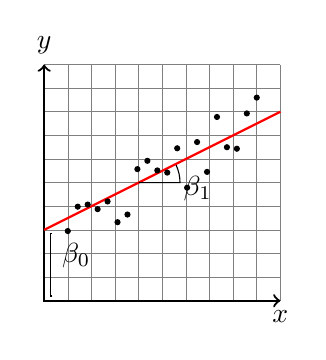
\begin{tikzpicture}[scale=0.15]
% background grid
\draw[step=2, gray, very thin] (-10,-10) grid (10,10);
%axis
\draw[thick, <->] (-10,10) node[anchor=south] {$y$} -- (-10,-10) -- (10,-10) node[anchor=north] {$x$};
% regression line
\draw[red, thick] plot [domain=-10:10] (\x,{1 + 0.5 * \x});
% data points
\draw plot [only marks, mark=*, mark size=6, domain=-8:8, samples=20] (\x,{rnd * 5 - 1.5 + 0.5 * \x});
% beta0
\draw (-9.3,-9.6) -- (-9.5,-9.6) -- (-9.5,-4.3) -- (-9.3, -4.3) node[anchor=north west] {$\beta_0$};
% beta1
\draw (-2,0) -- (1.5,0) arc (0:25:3.5);
\draw (3,-0.5) node {$\beta_1$};
\end{tikzpicture}

\columnbreak

Equation:\\ $y_i = \beta_0 + \beta_1 x_{1i} + u_i$

\vspace*{1mm}

Estimation:\\ $\hat{y}_i = \hat{\beta}_0 + \hat{\beta}_1 x_{1i}$

\vspace*{1mm}

Where: \\ $\hat{\beta}_0 = \overline{y} - \hat{\beta}_1 \overline{x}$ \\ $\hat{\beta}_1 = \frac{Cov(y, x)}{Var(x)}$

\end{multicols}

\subsection*{Multiple regression model}

\setlength{\multicolsep}{0pt}
\setlength{\columnsep}{-40pt}
\begin{multicols}{2}

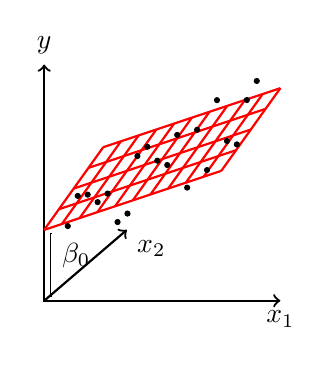
\begin{tikzpicture}[scale=0.15]
% axis
\draw[thick, ->] (-10,-10) -- (-3,-4) node[anchor=north west] {$x_2$};
\draw[thick, <->] (-10,10) node[anchor=south] {$y$} -- (-10,-10) -- (10,-10) node[anchor=north] {$x_1$};
% regression grid
\draw[red, thick] (-10,-4) -- (-5,3);
\draw[red, thick] (-8.5, -3.5) -- (-3.5,3.5);
\draw[red, thick] (-7, -3) -- (-2,4);
\draw[red, thick] (-5.5, -2.5) -- (-0.5,4.5);
\draw[red, thick] (-4, -2) -- (1,5);
\draw[red, thick] (-2.5, -1.5) -- (2.5,5.5);
\draw[red, thick] (-1, -1) -- (4,6);
\draw[red, thick] (0.5, -0.5) -- (5.5,6.5);
\draw[red, thick] (2, 0) -- (7,7);
\draw[red, thick] (3.5, 0.5) -- (8.5,7.5);
\draw[red, thick] (5, 1) -- (10,8);
\draw[red, thick] (-10, -4) -- (5, 1);
\draw[red, thick] (-8.75, -2.25) -- (6.25,2.75);
\draw[red, thick] (-7.5, -0.5) -- (7.5,4.5);
\draw[red, thick] (-6.25, 1.25) -- (8.75,6.25);
\draw[red, thick] (-5,3) -- (10,8);
% data points
\draw plot [only marks, mark=*, mark size=6, domain=-8:8, samples=20] (\x,{rnd * 6.5 - 1.5 + 0.5 * \x});
% beta0
\draw (-9.3,-9.6) -- (-9.5,-9.6) -- (-9.5,-4.3) -- (-9.3, -4.3) node[anchor=north west] {$\beta_0$};
\end{tikzpicture}

\columnbreak

Equation: \\ $y_i = \beta_0 + \beta_1 x_{1i} + ... + \beta_k x_{ki} + u_i$

\vspace*{1mm}

Estimation: \\ $\hat{y}_i = \hat{\beta}_0 + \hat{\beta}_1 x_{1i} + ... + \hat{\beta}_k x_{ki}$

\vspace*{1mm}

Where: \\ $\hat{\beta}_0 = \overline{y} - \hat{\beta}_1 \overline{x}_1 - ... - \hat{\beta}_k \overline{x}_k$ \\ $\hat{\beta}_j = \frac{Cov(y, \text{residualized } x_j)}{Var(\text{residualized } x_j)}$

\vspace*{1mm}

Matrix form: $\hat{\beta} = (X^T X)^{-1} (X^T Y)$

\end{multicols}

\subsection*{Interpretation of coefficients}

\scalebox{0.872}{
\begin{tabular}{ c c c c }
	Model & Dependent & Independent & $\beta_1$ interpretation \\
	\hline
	Level-level & $y$ & $x$ & $\Delta y = \beta_1 \Delta x$ \\ 
	Level-log & $y$ & $log(x)$ & $\Delta y = (\beta_1/100) \% \Delta x$ \\  
	Log-level & $log(y)$ & $x$ & $\% \Delta y = (100 \beta_1) \Delta x$ \\
	Log-log & $log(y)$ & $log(x)$ & $\% \Delta y = \beta_1 \% \Delta x$ \\
	Quadratic & $y$ & $x + x^2$ & $\Delta y = (\beta_1 + 2 \beta_2 x) \Delta x$ \\
\end{tabular}
}

\subsection*{Error measures}

Sum of Sq. Resid.: $SSR = \sum_{i=1}^n \hat{u}_i^2 = \sum_{i=1}^n (y_i - \hat{y}_i)^2$

Expl. Sum of Sq.: $SSE = \sum_{i=1}^n (\hat{y}_i - \overline{y}_i)^2$

Tot. Sum of Sq.: $SST = \sum_{i=1}^n (y_i - \overline{y}_i)^2 = SSE + SSR$

Standard error ($se$) of the regression: $\hat{\sigma} = \sqrt{\frac{\sum_{i=1}^n \hat{u}_i^2}{n-k-1}}$

Sqrt. of the Quadratic Mean Error: $\sqrt{\frac{\sum_{i=1}^n (\hat{u}_i - \overline{u})^2}{n}}$

Absolute Mean Error: $\frac{\sum_{i=1}^n |\hat{u}_i|}{n}$

Mean Percentage Error: $\frac{\sum_{i=1}^n |\hat{u}_i / y_i|}{n} 100$

\columnbreak

\subsection*{R-squared}

Is a measure of the goodness of the fit (how the OLS fits to the data):

$R^2 = \frac{\sum_i^n (\hat{y}_i - \overline{y}_i)^2}{\sum_i^n (y_i - \overline{y}_i)^2} = 1 - \frac{\sum_i^n \hat{u}_i^2}{nS_y^2}$

\begin{itemize}[leftmargin=*]
\item Measures the percentage of variation of $y$ that is linearly explained by the variations of $x$'s.
\item Takes values between 0 (no linear explanation of the variations of $y$) and 1 (total explanation of the variations of $y$).
\item When the number of regressors increment, the value of the r-squared increments as well, whatever the new variables are relevant or not.
\end{itemize}

To eliminate the last point, there is an r-squared corrected by degrees of freedom:

$\overline{R}^2 = 1 - \frac{n-1}{n-k-1} \frac{\sum_{i=1}^n \hat{u}_i^2}{\sum_{i=1}^n (y_i - \overline{y}_i)^2} = 1 - \frac{n-1}{n-k-1} (1-R^2)$

For big sample sizes: $\overline{R}^2 \approx R^2$

\section*{Hypothesis testing}
\subsection*{The basics of hypothesis testing}

An hypothesis test is a rule designed to explain from a sample, if exist evidence or not to reject an hypothesis that is made of one or more population parameters.

Elements of an hypothesis contrast:

\begin{itemize}[leftmargin=*]
\item Null hypothesis ($H_0$): is the hypothesis that you want to contrast.
\item Alternative hypothesis ($H_1$): is the hypothesis that cannot be rejected when the null hypothesis is rejected.
\item Statistic of contrast: is a random variable with a known distribution that allow us to see if we reject (or not) the null hypothesis.
\item Significance level ($\alpha$): is the probability of rejecting the null hypothesis being true (type I error). Is chosen by who conduct the contrast. Commonly is 0.10, 0.05, 0.01 or 0.001
\item Critic value: is the value that, for a determined value of $\alpha$, determines the reject (or not) of the null hypothesis.
\item p-value: is the highest level of significance for what we do not reject (accept) the null hypothesis ($H_0$).
\end{itemize}

\textbf{The rule is}: if p-value is lower than $\alpha$, there is evidence at that given $\alpha$ to reject the null hypothesis (accept the alternative instead).

\subsection*{Individual contrasts}

Under the premise of normality of the residuals, contrast if a given parameter is significantly different from a given value.

\begin{itemize}[leftmargin=*]
\item $H_0: \beta_j = \theta$
\item $H_1: \beta_j \neq \theta$
\end{itemize}

Under $H_0$:

$t = \frac{\hat{\beta}_j - \beta_j}{se(\hat{\beta}_j)} \sim t_{n-k-1, \alpha/2}$

If $\mid t \mid > t_{n-k, \alpha/2}$ there is evidence to reject the null hypothesis.

\textbf{Individual significance contrasts} - contrast if a given parameter is significantly different from zero.

\begin{itemize}[leftmargin=*]
\item $H_0: \beta_j = 0$
\item $H_1: \beta_j \neq 0$
\end{itemize}

Under $H_0$:

$t = \frac{\hat{\beta}_j - 0}{se(\hat{\beta}_j)} \sim t_{n-k-1, \alpha/2}$

If $\mid t \mid > t_{n-k-1, \alpha/2}$ there is evidence to reject the null hypothesis.

\section*{Confidence intervals}

Under the normality of the residuals requirement, the confidence intervals at ($1 - \alpha$) confidence can be calculated:

$\hat{\beta}_j \mp t_{n-k-1, \alpha/2} se(\hat{\beta}_j)$

\section*{The F contrast}

It uses a non restricted model and a restricted model to do assumptions about the parameters.

\begin{itemize}[leftmargin=*]
\item Non restricted model: is the model on which we want to make the hypothesis contrast.
\item Restricted model: is the model on which the hypothesis that we want to contrast have been imposed.
\end{itemize}

Then, looking at the errors, there are:

\begin{itemize}[leftmargin=*]
\item $\sum_{i=1}^n \hat{u}_{nr}^2$: is the Sum of Sq. Resid. of the non restricted model ($SSR_{nr}$).
\item $\sum_{i=1}^n \hat{u}_r^2$: is the Sum of Sq. Resid of the restricted model ($SSR_r$).
\end{itemize}

Then: $F = \frac{SSR_r - SSR_{nr}}{SSR_{nr}} \frac{(n-K-1)}{q} \sim F_{q, n-K-1}$

Where $K$ is the number of parameters of the non restricted model and $q$ is the number of linear hypothesis.

When $F_{q, n-K-1} < F$, there is evidence to reject the null hypothesis.

\section*{Dummy variables and structural change}

Dummy (or binary) variables are used for qualitative information: sex, civil state, etc.

\begin{itemize}[leftmargin=*]
\item The dummy variables get the value of 1 in a given category, and 0 on the rest.
\item Dummy variables are used to analyze and modeling structural changes in the model parameters.
\end{itemize}

If a qualitative variable have $m$ categories, we only have to include ($m-1$) dummy variables.

\subsection*{Structural change}

We denominate structural changes to the modifications in the value of the parameters of the models for different sub-populations.

The position of the dummy variable matters:
\begin{itemize}[leftmargin=*]
\item On the constant, their associate parameter represents the difference in mean between the values.
\item On the parameters that determines the slope of the regression line, the associate parameter represents the difference in the effect between the values.
\end{itemize}

\textbf{The Chow's structural contrast}

When we want to analyze the existence of structural changes in all the model parameters, is more common to use a particular expression of the F contrast known as the Chow's contrast.

It defines two non restricted models (with structural change):

$y_i = \beta_0^A + \beta_1^A x_{1i} + ... + \beta_k^A x_{ki} + u_i$ from sub-sample A

$y_i = \beta_0^B + \beta_1^B x_{1i} + ... + \beta_k^B x_{ki} + u_i$ from sub-sample B

Restricted model (without structural change):

$y_i = \beta_0 + \beta_1 x_{1i} + ... + \beta_k x_{ki} + u_i$

With the restriction:

$H_0: \beta_j^A = \beta_j^B$ for $j=0,1,...,k$, there is no structural difference.

\begin{itemize}[leftmargin=*]
\item Be $SSR_{nr}$ the sum of the OLS square residuals of the non restricted model: $SSR_{nr} = SSR_A + SSR_B$
\item Be $SSR_r$ the sum of the OLS square residuals of the restricted model.
\end{itemize}

Then:

$F = \frac{SSR_r - SSR_{nr}}{SSR_{nr}} \frac{n-2(k+1)}{k+1} \sim F_{k+1,n-2(k+1)}$

If $F_{q, n-K-1} < F$, there is evidence to reject the null hypothesis.

\section*{Multicollinearity}

If there is exact multicolineality, the equation system of OLS cannot be solved due to infinite solutions.

\begin{itemize}[leftmargin=*]
\item Approximate multicollinearity: when one or more variables are almost a constant or there is a linear relation between them. In this context, there is not a problem, given the classic requirements of OLS, and the inference is valid. But, there are some empiric consequences of this:
\begin{itemize}[leftmargin=*]
\item Small sample variations can induce to big variations in the OLS estimations.
\item The variance of the OLS estimator of the $x$'s that are collinear $Var(\hat{\beta}_j)$ increments, then, the inference of the parameter is affected $\rightarrow$ The estimation of the parameter is very imprecise (big confidence interval).
\end{itemize}
\end{itemize}

Calculating the Variance Inflation Factor to analyze multicollinearity problems:

$VIF(\hat{\beta}_j) = \frac{1}{1-R_j^2}$

Indicates the increment of $Var(\hat{\beta}_j)$ because of the multicollinearity.

\begin{itemize}[leftmargin=*]
\item If it is bigger than 10, indicates that there are multicollinearity problems.
\item From 4 onwards, it is advisable to analyze in more detail if there might be
multicollinearity.
\end{itemize}

One typical characteristic of multicollinearity is that the regression coefficients of the model are not individually different from zero (because the high variances), but jointly they are different from zero.

\section*{Heteroscedasticity}

The residuals $u_i$ of the population regression function do not have the same variance $\sigma^2$:

$Var(u|x) = Var(y|x) \neq \sigma^2$

\subsection*{Consequences}

\begin{itemize}[leftmargin=*]
\item The estimators still are unbiased.
\item The estimators still are consistent.
\item The variance estimations of the estimators is biased: the construction of confidence intervals and the hypothesis contrast are not reliable.
\end{itemize}

In this context, OLS is not an unbiased lineal estimator of minimum variance. There is an alternate unbiased lineal estimator of minimum variance denominated estimator of least weighted squares (OLWS) or least generalized squares (LGS).

\subsection*{Detection}

Plots. Look for structures in plots with the square residuals) and contrasts: Park test, Goldfield-Quandt, Bartlett, Breush-Pagan, CUSUMQ, Spearman, White.

White test null hypothesis:

$H_0 = Homoscedasticity$

\subsection*{Correction}

\begin{itemize}[leftmargin=*]
\item When the variance structure is known, use weighted least squares.
\item When the variance structure is not known: make assumptions of the possible structure and apply weighted least squares (factible weighted least squares).
\item Supposing that $\sigma_i^2$ is proportional to $x_i^2$, divide by $x_i$.
\item New model specification, for example, logarithmic transformation.
\item Standard errors with heteroscedasticity corrected by the White's method.
\end{itemize}

\section*{Auto-correlation}

The "natural" context of this phenomena is in temporal series.

The residual of any observation, $u_i$ is correlated with the residual of any other observation. The observations are not independent $E(u_i,u_j) \neq 0; i \neq j$

\subsection*{Consequences}

OLS estimators are not lineal, not efficient, and are biased.

Because OLS estimators are not efficient, variance estimations of the estimators are biased, hypothesis contrast and confidence intervals are not reliable.

\subsection*{Detection}

\begin{itemize}[leftmargin=*]
\item Graphic residual analysis. There are auto-correlation structures that can be identified in a plot. For example: 
\end{itemize}

\setlength{\multicolsep}{0pt}
\begin{multicols}{3}

AR:

\vspace{2.5pt}

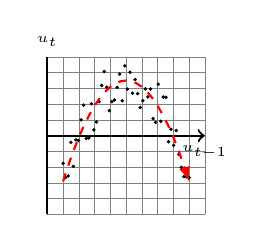
\begin{tikzpicture}[scale=0.1]
\draw[step=2, gray, very thin] (-10,-10) grid (10,10);
\draw[thick,->] (-10,0) -- (10,0) node[anchor=north] {$\scriptscriptstyle u_{t-1}$};
\draw[thick,-] (-10,-10) -- (-10,10) node[anchor=south] {$\scriptscriptstyle u_t$};
\draw plot [only marks, mark=*, mark size=4, domain=-8:8, samples=50] (\x,{rnd * 6 + (-2 * (\x)^2 + 40) * 0.1});
\draw[thick, dashed, red, -latex] plot [domain=-8:8] (\x,{3 + (-2 * (\x)^2 + 40) * 0.1});
\end{tikzpicture}

\columnbreak

AR(+):

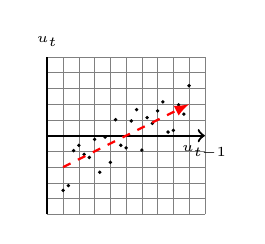
\begin{tikzpicture}[scale=0.1]
\draw[step=2, gray, very thin] (-10,-10) grid (10,10);
\draw[thick,->] (-10,0) -- (10,0) node[anchor=north] {$\scriptscriptstyle u_{t-1}$};
\draw[thick,-] (-10,-10) -- (-10,10) node[anchor=south] {$\scriptscriptstyle u_t$};
\draw plot [only marks, mark=*, mark size=4, domain=-8:8, samples=25] (\x,{rnd * 6 + 0.5 * \x - 3});
\draw[thick, dashed, red, -latex] plot [domain=-8:8] (\x,{3 + 0.5 * \x - 3});
\end{tikzpicture}

\columnbreak

AR(-):

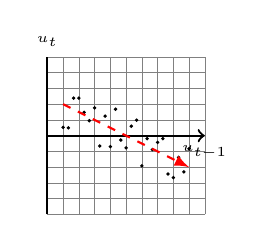
\begin{tikzpicture}[scale=0.1]
\draw[step=2, gray, very thin] (-10,-10) grid (10,10);
\draw[thick,->] (-10,0) -- (10,0) node[anchor=north] {$\scriptscriptstyle u_{t-1}$};
\draw[thick,-] (-10,-10) -- (-10,10) node[anchor=south] {$\scriptscriptstyle u_t$};
\draw plot [only marks, mark=*, mark size=4, domain=-8:8, samples=25] (\x,{rnd * 6 - 0.5 * \x - 3});
\draw[thick, dashed, red, -latex] plot [domain=-8:8] (\x,{3 - 0.5 * \x - 3});
\end{tikzpicture}

\end{multicols}

\begin{itemize}[leftmargin=*]
\item Formal contrasts: Breusch-Godfrey. It allows:
\begin{itemize}[leftmargin=*]
\item Dynamic models.
\item $u_t$ that follows an auto-regressive model or $\rho$ order.
\item Moving averages of the error term.
\end{itemize}
\end{itemize}

$H_0: No auto-correlation$

$H_1: u_t \sim AR(\rho)$ or $u_t \sim MA(q)$

\subsection*{Correction}



\section*{Prediction}

Two types of prediction:

\begin{itemize}[leftmargin=*]
\item Prediction of the mean value of $y$ for a specific value of $x$.
\item Prediction of an individual value of $y$ for a specific value of $x$.
\end{itemize}

If the values of the variables ($x$) approximate to the mean values ($\overline{x}$), the confidence interval amplitude will be less. 





\end{multicols}
\end{document}
